\documentclass[11pt]{article}

\usepackage{mathtools}
\usepackage{float}
\usepackage{amssymb}
\usepackage{amsmath}
\usepackage{amsthm}
\usepackage{hyperref}
\usepackage{microtype}
\usepackage{graphicx}
\usepackage{blkarray}
\usepackage{pgfplots}
\pgfplotsset{compat=1.15}
\usepackage{mathrsfs}
\usetikzlibrary{arrows}
\graphicspath{ {./img/} }

\setlength{\parindent}{0cm}
\let\emptyset\varnothing

\title{\textbf{MATH 2135 Linear Algebra} \\ Chapter 6 Inner Product Spaces}
\author{Alyssa Motas}

\begin{document}

    \maketitle

    \pagebreak

    \tableofcontents

    \pagebreak

    \section{6.A Inner Products and Norms}

    To motivate the concept of inner product, think of vectors in \(\mathbb{R}^2\) and \(\mathbb{R}^3\) as arrows with initial point at the origin. The length of a vector $x$ in \(\mathbb{R}^2\) or \(\mathbb{R}^3\) is called the \text{\emph{norm}} of $x$, denoted \(||x||\). Thus for \(x = (x_1, x_2) \in \mathbb{R}^2\), we have \(||x|| = \sqrt{x_1^2 + x_2^2}\). The generalization to \(\mathbb{R}^n\) is: we defined the norm of \(x = (x_1, \dots, x_n) \in \mathbb{R}^n \) by \[||x|| = \sqrt{x_1^2 + \dots + x_n^2.}\] 
    
    \begin{figure}[H]
        \centering
        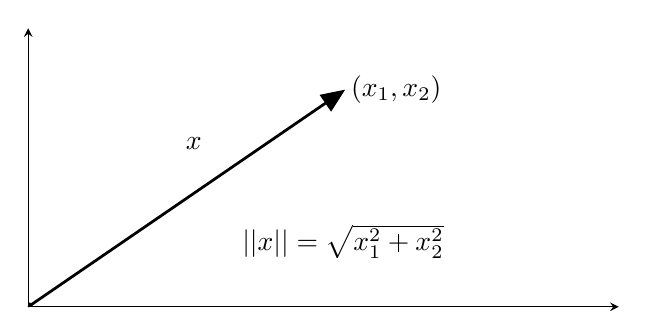
\begin{tikzpicture}[line cap=round,line join=round,>=triangle 45,x=1cm,y=1cm,scale=1]
            \begin{axis}[
            x=15cm,y=15cm,
            axis lines=middle,
            xmin=0,
            xmax=0.5,
            ymin=0,
            ymax=0.23585344119169532,
            ticks=none]
            \clip(-0.057132465392472714,-0.04075298644022664) rectangle (0.38291015883609275,0.23585344119169532);
            \draw [->,line width=1pt] (0,0) -- (0.2683348542861568,0.18381668611374563);
            \draw (0.12526118107302275,0.1517683147773752) node[anchor=north west] {$x$};
            \draw (0.2651441823780563,0.2039704573213492) node[anchor=north west] {$(x_1, x_2)$};
            \draw (0.1729420398340814,0.07787469228457479) node[anchor=north west] {$||x|| = \sqrt{x_1^2 + x_2^2}$};
            \begin{scriptsize}
            \draw [fill=black] (0,0) circle[radius=1.5pt];
            \end{scriptsize}
            \end{axis}
        \end{tikzpicture}
    \end{figure}
    
    The norm is not linear on \(\mathbb{R}^n\).

    \subsection{Definition of dot product}

    For \(x,y \in \mathbb{R}^n\), the \textbf{\emph{dot product}} of $x$ and $y$, denoted \(x \cdot y\), is defined by \[x \cdot y = x_1 y_1 + \dots + x_n y_n\] where \(x = (x_1, \dots, x_n)\) and \(y = (y_1, \dots, y_n)\). Note that the dot product of two vectors in \(\mathbb{R}^n\) is a number, not a vector. 

    \vspace{1em}

    An inner product is a generalization of the dot product. Recall that if \(\lambda = a + bi\), where \(a,b \in \mathbb{R}\), then 
    \begin{itemize}
        \item the absolute value of \(\lambda\), denoted \(|\lambda|\), is defined by \(|\lambda| = \sqrt{a^2 + b^2}\);
        \item the complex conjugate of \(\lambda\), denoted \(\overline{\lambda}\), is defined by \(\overline{\lambda} = a - bi\);
        \item \(|\lambda|^2 = \lambda \overline{\lambda}\).
    \end{itemize}
    For \(z = (z_1, \dots, z_n) \in \mathbb{C}^n\), we define the norm of $z$ by \[||z|| = \sqrt{|z_1|^2 + \dots + |z_n|^2}.\] The absolute values are needed because we want \(||z||\) to be nonegative number. Note that \[||z||^2 = z_1 \overline{z_1} + \dots + z_n \overline{z_n}.\] We want to think of \(||z||^2\) as the inner product of $z$ with itself. The equation above suggests that the inner product of \(w = (w_1, \dots, w_n) \in \mathbb{C}^n\) with $z$ should equal \[w_1 \overline{z_1} + \dots + w_n \overline{z_n}.\] If the roles of $w$ and $z$ were interchanged, the expression above would be its complex conjugate. We should expect that the inner product of $w$ with $z$ equals the complex conjugate of the inner product of $z$ with $w$. 

    \subsection{Definition of inner product}

    An \textbf{\emph{inner product}} on $V$ is a function that takes each ordered pair \((u,v)\) of elements of $V$ to a number \(\langle u,v \rangle \in \textbf{F}\) and has the following properties:

    \begin{enumerate}
        \item[] \textbf{positivity} \[\langle v,v \rangle \geq 0 \text{ for all } v \in V;\]
        \item[] \textbf{definiteness} \[\langle v,v \rangle = 0 \text{ if and only if } v = 0;\]
        \item[] \textbf{additivity in first slot} \[\langle u + v, w \rangle = \langle u,w \rangle + \langle v,w \rangle \text{ for all } u,v,w \in V;\]
        \item[] \textbf{homogeneity in first slot} \[\langle \lambda u, v \rangle = \lambda \langle u,v \rangle \text{ for all } \lambda \in \textbf{F} \text{ and all } u,v \in V;\]
        \item[] \textbf{conjugate symmetry} \[\langle u,v \rangle = \overline{\langle v,v \rangle} \text{ for all } u,v \in V.\]
    \end{enumerate}

    Every real number equals its complex conjugate. If we are dealing with a real vector space, then the last condition can be \(\langle u,v \rangle = \langle v,u \rangle\) for all \(v,w \in V\). 

    \subsubsection{Examples}
    \begin{enumerate}
        \item[(a)] The \textbf{\emph{Euclidean inner product}} on \(\textbf{F}^n\) is defined by \[\langle (w_1, \dots, w_n), (z_1, \dots, z_n) \rangle = w_1 \overline{z_1} + \dots + w_n \overline{z_n}.\]
        \item[(b)] If \(c_1, \dots, c_n\) are positive numbers, then an inner product can be defined on \(\textbf{F}^n\) by \[\langle (w_1, \dots, w_n), (z_1, \dots, z_n) \rangle = c_1 w_1 \overline{z_1} + \dots + c_n w_n \overline{z_n}.\]  
        \item[(c)] An inner product can be defined on the vector space of continuous real-valued functions on the interval \([-1,1]\) by \[\langle f,g \rangle = \int_{-1}^{1} f(x) \overline{g(x)}dx.\] This is an inner product since for example: additivity in the left slot is defined as
        \begin{align*}
            \langle f+h, g \rangle &= \int_{-1}^{1} (f(x) + h(x)) \overline{g(x)} dx \\
                                   &= \int_{-1}^{1} f(x) \overline{g(x)} + \int_{-1}^{1} h(x) \overline{g(x)} dx \\
                                   &= \langle f,g \rangle + \langle h,g \rangle.
        \end{align*} 
        \item[(d)] An inner product can be defined on \(\mathcal{P}(\mathbb{R})\) by \[\langle p,q \rangle = \int_{0}^{\infty} p(x) q(x) e^{-x} dx.\]  
        \item[(e)] The dot product on \(\mathbb{R}^n\) \[\langle v,w \rangle = v \cdot w = x_1 y_1 + \dots + x_n y_n\] and \[\langle v,v \rangle = v \cdot v = x_1^2 + \dots + x_n^2 \geq 0.\]
    \end{enumerate}

    \subsection{Definition of inner product space}

    An \textbf{\emph{inner product space}} is a vector space $V$ along with an inner product on $V$. For the rest of this chapter, $V$ denotes an inner product space over \textbf{F}. 

    \subsection{Basic properties of an inner product}

    \begin{enumerate}
        \item[(a)] For each fixed \(u \in V\), the function that takes $v$ to \(\langle v,u \rangle\) is a linear map from $V$ to \textbf{F}.
        \begin{proof}
            \begin{itemize}
                \item \(f(v+v') = \langle v+ v', u \rangle = \langle v,u \rangle + \langle v', u \rangle = f(v) + f(v')\)
                \item \(f(\lambda v) = \dots = \lambda f(v).\)
            \end{itemize}
        \end{proof} 
        \item[(b)] \(\langle 0,u \rangle = 0\) for every \(u \in V\).
        \item[(c)] \(\langle u,0 \rangle = 0\) for every \(u \in V\).
        \item[(d)] \(\langle u,v+w \rangle = \langle u,v \rangle + \langle u,w \rangle\) for all \(u,v,w \in V\).  
        \begin{proof}
            This is additivity in the second slot.
            \begin{align*}
                \langle u,v+w \rangle &= \overline{\langle v+w, u \rangle} \\
                                      &= \overline{\langle v,u \rangle + \langle w, u \rangle} \\
                                      &= \overline{\langle v,u \rangle} + \overline{\langle w,u \rangle} \\
                                      &= \langle u,v \rangle + \langle u,w \rangle. 
            \end{align*}
        \end{proof} 
        \item[(e)] \(\langle u, \lambda v \rangle = \overline{\lambda} \langle u,v \rangle\) for all \(\lambda \in \textbf{F}\) and \(u,v \in V\).  
        \begin{proof}
            This is homogeneity in the second slot.
            \begin{align*}
                \langle u, \lambda v \rangle &= \overline{\langle \lambda v, u \rangle} \\
                                             &= \overline{\lambda \langle v,u \rangle} \\
                                             &= \overline{\lambda} \overline{\langle v, u \rangle} \\
                                             &= \overline{\lambda} \langle u,v \rangle. 
            \end{align*}
        \end{proof} 
    \end{enumerate}

    \subsection{Definition of norm, \(||v||\)}

    For \(v \in V\), the \textbf{\emph{norm}} of $v$, denoted \(||v||\), is defined by \[||v|| = \sqrt{\langle v,v \rangle} \geq 0.\] Note that \(||v||^2 = \langle v,v \rangle.\)

    \subsection{Basic properties of the norm}

    Suppose \(v \in V\).

    \begin{enumerate}
        \item[(a)] \(||v|| = 0\) if and only if \(v = 0\). 
        \item[(b)] \(||\lambda v|| = |\lambda | ||v||\) for all \(\lambda \in \textbf{F}\).  
    \end{enumerate}
    \begin{proof}
        \begin{enumerate}
            \item[(a)] The desired result holds because \(\langle v,v \rangle = 0\) if and only if \(v = 0\).
            \item[(b)] Suppose \(\lambda \in \textbf{F}\). then
            \begin{align*}
                ||\lambda v||^2 &= \langle \lambda v, \lambda v \rangle \\
                                &= \lambda \langle v, \lambda v \rangle \\
                                &= \lambda \overline{\lambda} \langle v,v \rangle \\
                                &= |\lambda|^2 || v || 2.
            \end{align*}   
            Taking square roots now gives the desired equality. 
        \end{enumerate}
    \end{proof}

    \subsection{Definition of orthogonal}

    Two vectors \(u,v \in V\) are called \textbf{\emph{orthogonal}} if \(\langle u,v \rangle = 0\). We write \(u \perp v\) to mean ``$u$ is orthogonal to $v$.''

    \subsection{Orthogonality and 0}
    \begin{enumerate}
        \item[(a)] 0 is orthogonal to every vector in $V$.
        \item[(b)] 0 is the only vector in $V$ that is orthogonal to itself. 
        \begin{proof}
            If \(v \in V\) and \(\langle v,v \rangle = 0\), then \(v = 0\) (by definition of inner product).
        \end{proof}   
        \item[(c)] \(u \perp v \Leftrightarrow v \perp u\)
        \item[(d)] \(u \perp w\) and \(v \perp w \Rightarrow (u+v) \perp w\)  .
        \item[(e)] \(u \perp w\) and \(\lambda \in \textbf{F} \Rightarrow (\lambda u) \perp w\).   
    \end{enumerate}

    The last two properties imply that the set \[w^{\perp} = \{v \mid v \perp w\}\] is a subspace of $V$, called the \emph{orthogonal complement of $V$}.

    \begin{figure}[H]
        \centering
        \definecolor{qqqqff}{rgb}{0,0,1}
        \definecolor{ccqqqq}{rgb}{0.8,0,0}
        \begin{tikzpicture}[line cap=round,line join=round,>=triangle 45,x=1cm,y=1cm, scale=1]
        \clip(-2.6180510577677225,-0.020004894937517982) rectangle (13.737835166148363,10.261142907693804);
        \draw [line width=1pt,color=ccqqqq] (2.0820772765971225,5.817064550395381)-- (4.541491327323378,1.9614141749671257);
        \draw [line width=1pt,color=ccqqqq] (4.541491327323378,1.9614141749671257)-- (7.0585367634417295,3.566131921468393);
        \draw [line width=1pt,color=ccqqqq] (7.0585367634417295,3.566131921468393)-- (4.672005783374561,7.145928391569146);
        \draw [line width=1pt,color=ccqqqq] (4.672005783374561,7.145928391569146)-- (2.0820772765971225,5.817064550395381);
        \draw [->,line width=1pt] (0.7180503154458768,2.7986640315826374) -- (7.374186675539191,6.105800965213908);
        \draw [->,line width=1pt] (1.2343543936921086,6.8035091790601685) -- (8.574244803354755,1.724193382259398);
        \draw [->,line width=1pt] (4.387995520277201,0.5241352544438309) -- (4.429858013107976,9.775746170045235);
        \draw [->,line width=1pt,color=ccqqqq] (4.354489862439656,4.605448460592127) -- (3.950679670128945,5.954629104885521);
        \draw [->,line width=1pt,color=ccqqqq] (4.354489862439656,4.605448460592127) -- (4.99907668567554,5.7050107678506174);
        \draw [->,line width=1pt,color=ccqqqq] (4.354489862439656,4.605448460592127) -- (5.38848129144999,4.536796950527268);
        \draw [->,line width=1pt,color=ccqqqq] (4.354489862439656,4.605448460592127) -- (4.789397282566221,3.5582930693504466);
        \draw [->,line width=1pt,color=ccqqqq] (4.354489862439656,4.605448460592127) -- (4.060511738424303,3.7080640715713886);
        \draw [->,line width=1pt,color=ccqqqq] (4.354489862439656,4.605448460592127) -- (3.251748326431215,4.8163694880063606);
        \draw [->,line width=1pt,color=qqqqff] (4.354489862439656,4.605448460592127) -- (7.215687518545484,7.352491792280982);
        \draw (6.917544928186012,7.794948574975387) node[anchor=north west] {$\text{\color{blue} w}$};
        \draw (2.7485008127164028,7.167901937275228) node[anchor=north west] {$\text{\color{red} $w^{\perp}$}$};
        \end{tikzpicture}
    \end{figure}

    \subsection{Pythagorean Theorem}

    Suppose $u$ and $v$ are orthogonal vectors in $V$. Then \[||u+v||^2 = ||u||^2 + ||v||^2.\]
    \begin{proof}
        We have
        \begin{align*}
            ||u+v||^2 &= \langle u+v, u+v \rangle \\
                      &= \langle u, u+v \rangle + \langle v, u+v \rangle \\
                      &= \langle u, u \rangle + \underbrace{\langle u,v \rangle + \langle v,u \rangle}_{0} + \langle v,v \rangle \\
                      &= \langle u,u \rangle + \langle v,v \rangle \\
                      &= ||u||^2 + ||v||^2,
        \end{align*}
        as desired.
    \end{proof}

    \subsection{Orthogonal Decomposition (Projection)}

    Given \(u,v \in V\), assuming \(v \neq 0\). Then we can write $u$ as a sum of two vectors, the first of which is parallel to $v$ and the second is orthogonal to $v$.

    \begin{figure}[H]
        \centering
        \definecolor{ccqqqq}{rgb}{0.8,0,0}
        \definecolor{qqqqff}{rgb}{0,0,1}
        \begin{tikzpicture}[line cap=round,line join=round,>=triangle 45,x=1cm,y=1cm,scale=1.5]
        \clip(0.4659165179786193,4.826312037466861) rectangle (6.3117730368156115,8.500959444542582);
        \draw [->,line width=1pt,color=qqqqff] (1.7151488232431262,5.751036310032376) -- (3.15785216765511,5.745073864066619);
        \draw [->,line width=1pt,color=qqqqff] (1.7151488232431262,5.751036310032376) -- (3.94,8.09151);
        \draw [->,line width=1pt,color=ccqqqq] (1.7151488232431262,5.751036310032376) -- (3.94178,5.75);
        \draw [->,line width=1pt,color=ccqqqq] (3.94178,5.75) -- (3.94,8.09151);
        \draw (2.350938136976971,5.665795349571387) node[anchor=north west] {$\text{\color{blue} $v$}$};
        \draw (2.438702301424262,7.18831281107005) node[anchor=north west] {$\text{\color{blue}$u$}$};
        \draw (3.1751581161341447,5.620005350729322) node[anchor=north west] {$\text{\color{red} $cv$}$};
        \draw (4.167274757712224,6.947915317149209) node[anchor=north west] {$\text{\color{red} $w$}$};
        \end{tikzpicture}
    \end{figure}

    Let \(c = \dfrac{\langle u,v \rangle}{||v||^2} = \dfrac{\langle u,v \rangle}{\langle v,v \rangle}\) and let \(w = u - cv\). Then \(\langle w,v \rangle = 0\) and \(u = cv + w\). 

    \begin{proof}
        We know \(u = cv + w\) holds by the definition of $w$. We also know that $cv$ is parallel to $v$ by the definition of ``parallel.'' To prove that $w$ is orthogonal to $v$, we can calculate:
        \begin{align*}
            \langle w,v \rangle &= \langle u-cv, v \rangle \\
                                &= \langle u,v \rangle - c \langle v,v \rangle \\
                                &= \langle u,v \rangle - \frac{\langle u,v \rangle}{\langle v,v \rangle} \langle v,v \rangle \\
                                &= \langle u,v \rangle - \langle u,v \rangle = 0.
        \end{align*}
        Therefore, \(w \perp v.\)
    \end{proof}

    \subsection{Cauchy-Schwarz Inequality}

    Suppose \(u,v \in V\). Then \[|\langle u,v \rangle| \leq ||u|| ||v||.\] This inequality is an equality if and only if one of $u,v$ is a scalar multiple of the other. 
    \begin{proof}
        Consider two cases:

        \vspace{1em}
        
        \emph{Case 1.} \(v = 0\) and in this case, \(\langle u,v \rangle = 0, ||u|| \cdot ||v|| = || u || \cdot 0 = 0.\) So the inequality holds.

        \vspace{1em}

        \emph{Case 2.} \(v \neq 0\). Consider the orthogonal decomposition \[u = cv + w\] where \(c = \dfrac{\langle u,v \rangle}{\langle v,v \rangle}\) and \(w = u - cv\). We know that \(w \perp v\). By Pythagoras' Theorem,
        \begin{align*}
            ||u||^2 &= ||cv||^2 + ||w||^2 \\
                    \geq& ||cv||^2 \\
                    &= |c|^2 ||v||^2 \\
                    &= \bigg|\frac{\langle u,v \rangle}{||v||^2}\bigg|^2 ||v||^2 \\
                    &= \frac{| \langle u,v \rangle |^2}{||v||^4} \cdot ||v||^2 \\
                    &= \frac{|\langle u,v \rangle|^2}{||v||^2}.
        \end{align*}
        We just proved that \[||u||^2 \geq \frac{| \langle u,v \rangle|^2}{||v||^2}.\] Multiply both sides of the equation by \(||v||^2\) and we get \[||u||^2 ||v||^2 \geq | \langle u,v \rangle |^2.\] Take the square root of both sides of the equation and we get \[||u|| \cdot ||v|| \geq | \langle u,v \rangle |\] which is the Cauchy-Schwarz inequality. 
    \end{proof}

    \subsubsection{Examples of the Cauchy-Schawrz Inequality}

    \begin{enumerate}
        \item[(a)] If \(x_1, \dots, x_n, y_1, \dots, y_n \in \mathbb{R}\) then \[|x_1 y_1 + \dots + x_n y_n|^2 \leq (x_1^2 + \dots + x_n^2)(y_1^2 + \dots + y_n^2).\] 
        \item[(b)] If $f,g$ are continuous real-valued functions on \([-1,1]\), then \[\bigg| \int_{-1}^{1} f(x)g(x)dx \bigg|^2 \leq \left( \int_{-1}^{1} (f(x))^2 dx \right) \left( \int_{-1}^{1} (g(x))^2 dx \right).\] 
    \end{enumerate}

    \subsection{Triangle Inequality}

    The Triangle Inequality implies that the shortest path between two points is a line segment. Suppose \(u,v \in V\). Then \[||u+v|| \leq ||u|| + ||v||.\] This inequality is an equality if and only if one of $u,v$ is a nonnegative multiple of the other.

    \begin{figure}[H]
        \centering
        \definecolor{qqqqff}{rgb}{0,0,1}
        \begin{tikzpicture}[line cap=round,line join=round,>=triangle 45,x=1cm,y=1cm,scale=1.5]
        \clip(1.1158324500362908,6.0266553337393765) rectangle (4.326145012145141,8.04462595861587);
        \draw [->,line width=1pt,color=qqqqff] (1.48474,6.54) -- (3.5338464403969887,7.779766962780057);
        \draw [->,line width=1pt,color=qqqqff] (1.48474,6.54) -- (2.8660756239502043,6.543436994044301);
        \draw [->,line width=1pt,color=qqqqff] (2.8660756239502043,6.543436994044301) -- (3.5338464403969887,7.779766962780057);
        \draw (2.0923374460824555,6.437374173278102) node[anchor=north west] {$u$};
        \draw (3.3559265289490594,7.080693988269881) node[anchor=north west] {$v$};
        \draw (2.1033991731005815,7.724356690741059) node[anchor=north west] {$u+v$};
        \end{tikzpicture}
    \end{figure}

    \begin{proof}
        We have 
        \begin{align*}
            ||u+v||^2 &= \langle u+v, u+v \rangle \\
                      &= \langle u,u \rangle + \langle u,v \rangle + \langle v,u \rangle + \langle v,v \rangle \\
                      &= \langle u,u \rangle + \langle u,v \rangle + \overline{\langle u,v \rangle} + \langle v,v \rangle \\
                      &\leq \langle u,u \rangle + 2 |\langle u,v \rangle| + \langle v,v \rangle \\
                      &\leq \langle u,u \rangle + 2 ||u|| ||v|| + \langle v,v \rangle \quad (\text{Cauchy-Schwarz}) \\
                      &= ||u||^2 + 2 ||u|| ||v|| + ||v||^2 \\
                      &= (||u|| + ||v||)^2
        \end{align*}
        Taking the square roots: \[|| u+v|| \leq ||u|| + ||v||,\] thus we get the triangle inequality.
    \end{proof}

    \subsection{Parallelogram Equality}
    
    In every parallelogram, the sum of the squares of the lengths of the diagonals equals the sum of the squares of the lengths of the four sides.

    Suppose $u,v \in V$. Then \[||u+v||^2 + ||u - v||^2 = 2(||u||^2 + ||v||^2).\]

    \begin{figure}[H]
        \centering
        \definecolor{qqqqff}{rgb}{0,0,1}
        \begin{tikzpicture}[line cap=round,line join=round,>=triangle 45,x=1cm,y=1cm, scale=5]
        \clip(1.4054755144183175,6.3261733476284885) rectangle (3.805268705098164,7.634659537331268);
        \draw [->,line width=1pt,color=qqqqff] (1.712547506177378,6.697110503175739) -- (2.9356517789417698,6.783031051262492);
        \draw [->,line width=1pt,color=qqqqff] (1.712547506177378,6.697110503175739) -- (3.0973845753403673,7.543680609324636);
        \draw [->,line width=1pt,color=qqqqff] (1.712547506177378,6.697110503175739) -- (1.9955798998749232,7.392056112700953);
        \draw [->,line width=1pt,color=qqqqff] (1.9955798998749232,7.392056112700953) -- (2.9356517789417698,6.783031051262492);
        \draw [->,line width=1pt,color=qqqqff] (2.9356517789417698,6.783031051262492) -- (3.0973845753403673,7.543680609324636);
        \draw [->,line width=1pt,color=qqqqff] (1.9955798998749232,7.392056112700953) -- (3.0973845753403673,7.543680609324636);
        \draw (2.2654536225666435,6.6692247241029525) node[anchor=north west] {$u$};
        \draw (2.2638871779252074,6.969982095258647) node[anchor=north west] {$u+v$};
        \draw (1.709365774856888,7.140724561175161) node[anchor=north west] {$v$};
        \draw (2.29364962611249,7.35532747705188) node[anchor=north west] {$u-v$};
        \draw (3.098802171810559,7.1814521218524945) node[anchor=north west] {$v$};
        \draw (2.4628256473875707,7.599692841115882) node[anchor=north west] {$u$};
        \end{tikzpicture}
    \end{figure}

    \begin{proof}
        We have 
        \begin{align*}
            ||u+v||^2 + ||u-v||^2 &= \langle u+v, u+v \rangle + \langle u-v, u-v \rangle \\
                                  &= ||u||^2 + ||v||^2 + \langle u,v \rangle + \langle v,u \rangle \\
                                  &\quad + ||u||^2 + ||v||^2 - \langle u,v \rangle - \langle v,u \rangle \\
                                  &= 2(||u||^2 + ||v||^2),
        \end{align*}
        as desired.
    \end{proof}

    \pagebreak

    \section{6.B Orthonormal Bases}

    \subsection{Definition of orthonormal}

    \begin{itemize}
        \item A list of vectors is called \textbf{\emph{orthonormal}} if each vector in the list has norm 1 and is orthogonal to all the other vectors in the list.
        \item In other words, a list \(e_1, \dots, e_m\) of vectors in $V$ is orthonormal if 
        \begin{equation*}
            \langle e_j, e_k \rangle = \begin{cases}
                1 & \text{if } j = k, \\
                0 & \text{if } j \neq k.
            \end{cases}
        \end{equation*}
    \end{itemize}

    \subsubsection{Examples}

    \begin{itemize}
        \item The standard basis in \(\textbf{F}^n\) is an orthonormal list. 
        \item In \(\mathbb{R}^2\), we have \[v_1 = \begin{bmatrix}
            1 \\ 0 \\ 0
        \end{bmatrix}, v_2 = \begin{bmatrix}
            0 \\ 1 \\ 1
        \end{bmatrix}, v_3 = \begin{bmatrix}
            0 \\ 1 \\ -1
        \end{bmatrix}.\] \(v_1, v_2, v_3\) is orthogonal but \emph{not} orthonormal. 

        \item In \(\mathbb{R}^3\), we have \[w_1 = \begin{bmatrix}
            1 \\ 0 \\ 0
        \end{bmatrix}, w_2 = \frac{1}{\sqrt{2}} \begin{bmatrix}
            0 \\ 1 \\ 1
        \end{bmatrix}, w_3 = \frac{1}{\sqrt{2}} \begin{bmatrix}
            0 \\ 1 \\ -1
        \end{bmatrix}.\] \(w_1, w_2, w_3\) is orthonormal. 
    \end{itemize}

    \emph{Note:} If \(v_1, \dots, v_n\) is orthogonal and all are non-zero, then \[\frac{v_1}{||v_1||}, \frac{v_2}{||v_2||}, \dots, \frac{v_n}{||v_n||}\] is orthonormal. 

    \subsection{The norm of an orthonormal linear combination}

    If \(e_1, \dots, e_m\) is an orthonormal list of vectors in $V$, then \[||a_1 e_1 + \dots + a_m e_m ||^2 = |a_1 |^2 + \dots + |a_m|^2\] for all \(a_1, \dots, a_m \in \textbf{F}\). 

    \begin{proof}
        \begin{align*}
            ||v||^2 &= \langle v,v \rangle \\
                    &= \langle a_1 e_1 + \dots + a_n e_n, a_1 e_1 + \dots + a_n e_n \rangle \\
                    &= a_1 \overline{a_1} \langle e_1, e_1 \rangle + a_1 \overline{a_2} \langle e_1, e_2 \rangle + \dots + a_1 \overline{a_n} \langle e_1, e_n \rangle \\
                    & \quad + a_2 \overline{a_1} \langle e_2, e_1 \rangle + a_2 \overline{a_3} \langle e_2, e_3 \rangle + \dots + a_2 \overline{a_n} \langle e_2, e_n \rangle \\
                    & \quad + \dots \\
                    & \quad + a_n \overline{a_1} \langle e_n, e_1 \rangle + a_n \overline{a_2} \langle e_n, e_2 \rangle + \dots + a_n \overline{a_n} \langle e_n, e_n \rangle \\
                    &= a_1 \overline{a_1} + a_2 \overline{a_2} + \dots + a_n \overline{a_n} \\
                    &= |a_1|^2 + |a_2|^2 + \dots + |a_n|^2.
        \end{align*}
    \end{proof}

    \subsection{An orthonormal list is linearly independent}
    
    Every orthonormal list of vectors is linearly independent. 
    \begin{proof}
        Let \(e_1, \dots, e_n\) be orthonormal. Take any \(a_1, \dots, a_n\) and assume \[a_1 e_1 + \dots + a_n e_n = 0.\] We need to show that \(a_i = 0\) for all $i$. Consider any index $i$ and we have 
        \begin{align*}
            0 = \langle 0, e_i \rangle &= \langle a_1 e_1 + \dots + a_n e_n, e_i \rangle \\
                                       &= a_1 \langle e_1, e_i \rangle + a_2 \langle e_2, e_i \rangle + \dots + a_i \langle e_i, e_i \rangle + \dots + a_n \langle e_n, e_i \rangle \\
                                       &= 0 a_1 + 0 a_2 + \dots + 1 a_1 + \dots + 0 a_n \\
                                       &= a_i.
        \end{align*}
        Since $i$ was arbitrary, we have \(a_1 = 0, \dots, a_n = 0\) as desired. 
    \end{proof}

    \subsection{Definition of orthonormal basis}

    An \textbf{\emph{orthonormal basis}} of $V$ is an orthonormal list of vectors in $V$ that is also a basis of $V$. For example, the standard basis is an orthonormal basis of \(\textbf{F}^n\). 

    \subsection{An orthonormal list of the right length is an orthonormal basis}

    Every orthonormal list of vectors in $V$ with length dim $V$ is an orthonormal basis of $V$. 

    \begin{proof}
        Since an orthonormal list is linearly independent, any such list must be linearly independent as well; because it has the right length, it is a basis. 
    \end{proof}

    \subsubsection{Example}

    Show that \[\frac{1}{2} \begin{bmatrix}
        1 \\ 1 \\ 1 \\ 1
    \end{bmatrix}, \frac{1}{2}\begin{bmatrix}
        1 \\ 1 \\ -1 \\ 1
    \end{bmatrix}, \frac{1}{2} \begin{bmatrix}
        1 \\ -1 \\ -1 \\ 1
    \end{bmatrix}, \frac{1}{2} \begin{bmatrix}
        -1 \\ 1 \\ -1 \\ 1
    \end{bmatrix}\] is an orthonormal basis of \(\textbf{F}^4\).

    \begin{proof}[\unskip\nopunct]
        \emph{Solution:} We have \[\bigg| \bigg| \left(\frac{1}{2}, \frac{1}{2}, \frac{1}{2}, \frac{1}{2} \right) \bigg| \bigg| = \sqrt{\left(\frac{1}{2}\right)^2 + \left(\frac{1}{2}\right)^2 + \left(\frac{1}{2}\right)^2 + \left(\frac{1}{2}\right)^2} = 1.\] Similarly, the other three vectors also have norm 1. The inner product of any two distinct vectors in the list above equals 0. Thus, the list above is orthonormal. Because we have an orthonormal list of length four in the four-dimensional vector space \(\textbf{F}^4\), this list is an orthonormal basis. 
    \end{proof}

    \subsection{Writing a vector as linear combination of orthonormal basis}

    Suppose \(e_1, \dots, e_n\) is an orthonormal basis of $V$ and \(v \in V\). Then \[v = \langle v, e_1 \rangle e_1 + \dots + \langle v, e_n \rangle e_n\] and \[||v||^2 = |\langle v, e_1 \rangle|^2 + \dots + |\langle v, e_n \rangle |^2. \]

    \begin{proof}
        Because \(e_1, \dots, e_n\) is a basis of $V$, there exist coordinates \(a_1, \dots, a_m\) such that \[v = a_1 e_1 + \dots + a_n e_n.\] Then 
        \begin{align*}
            \langle v, e_i \rangle &= \langle a_1, e_1 + \dots a_n e_n, e_i \rangle \\
                                   &= a_1 \langle e_1, e_i \rangle + \dots + a_n \langle e_n, e_i \rangle \\
                                   &= a_i.
        \end{align*}
        Plugging \(a_i = \langle v, e_i \rangle\) into $v$, we get \[v = \langle v,e_1 \rangle e_1 + \dots + \langle v,e_n \rangle e_n.\] The second claim follows from the fact that the norm of an orthonormal linear combination. 
    \end{proof}

    \subsection{Fourier coefficients}

    Let \(e_1, \dots, e_n\) be an orthonormal basis, and let \(v \in V\). In the formula, \[v = \langle v, e_1 \rangle e_1 + \dots + \langle v, e_n \rangle e_n\] the coefficients \(\langle v, e_1 \rangle, \dots, \langle v, e_n \rangle\) are the \textbf{Fourier coefficients} of $v$. 

    \vspace{1em}

    \emph{Note:} Almost the same trick works if \(e_1, \dots, e_n\) is an orthogonal basis (instead of an orthonormal one). In that case, the formula changes slightly as follows: When \(v = a_1 e_1 + \dots + a_n e_n\) then we get 
    \begin{align*}
        \langle v, e_i \rangle &= \langle a_1 e_1 + \dots + a_n e_n, e_i \rangle \\
                               &= a_1 \langle e_1, e_i \rangle + \dots + a_i \langle e_i, e_i \rangle + \dots + a_n \langle e_n, e_i \rangle \\
                               &= a_i \langle e_i, e_i \rangle.
    \end{align*}
    Then the formula for the Fourier coeffiecients becomes \[a_i = \frac{\langle v, e_i \rangle}{\langle e_i, e_i \rangle}\] and so we have \[v = \frac{\langle v, e_1 \rangle}{\langle e_1, e_1 \rangle} e_1 + \dots + \frac{\langle v, e_n \rangle}{\langle e_n, e_n \rangle} e_n\] which are the Fourier coefficients for orthogonal basis. 

    \subsection{Existence of orthonormal basis}

    Every finite-dimensional inner product space has an orthonormal basis. (And therefore, it also has an orthonormal basis as well, by normalizing the basis vector.)

    \begin{proof}
        Since $V$ is finite-dimensional, it has some basis, say \(v_1, \dots, v_n\). However, this basis may not be orthogonal. We will give a procedure for ``turning'' \(v_1, \dots, v_n\) into an orthogonal basis \(w_1, \dots, w_n\). (The Gram-Schmidt Procedure)
    \end{proof}

    \subsection{Gram-Schmidt Procedure}

    \emph{Note:} This version is different than the one in 6.31. I compute an orthogonal basis and Axler computes and orthonormal basis. Axler's computation uses a lot of square roots, and mine does not!

    \vspace{1em}

    We compute:
    \begin{align*}
        w_1 &= v_1 \\
        w_2 &= v_2 - \frac{\langle v_2, w_1 \rangle}{\langle w_1, w_1 \rangle} w_1 \\
        w_3 &= v_3 - \frac{\langle v_3, w_1 \rangle}{\langle w_1, w_1 \rangle} w_1 - \frac{\langle v_3, w_2 \rangle}{\langle w_2, w_2 \rangle} w_2 \\
        &\vdots \\
        w_n &= v_n - \frac{\langle v_n, w_1 \rangle}{\langle w_1, w_1 \rangle} w_1 - \dots - \frac{\langle v_n, w_{n-1} \rangle}{\langle w_{n-1}, w_{n-1} \rangle} w_{n-1}
    \end{align*}

    \emph{Claim:} \(w_1, \dots, w_n\) is an orthogonal basis of $V$.

    \begin{proof}
        To prove the claim above, we must show that
        \begin{enumerate}
            \item \(w_1,\dots, w_n\) are orthogonal.
            \item span(\(w_1, \dots, w_n\)) \( = \text{span}(v_1, \dots, v_n)\) 
        \end{enumerate}

        For (1), we can prove by induction on $n$.
        \begin{itemize}
            \item Base case: \(n=1\). Then $w_1$ is an orthogonal list of vectors (because there is only one vector).
            \item Induction step: By the induction hypotheses, \(w_1, \dots, w_{n-1}\) are orthogonal. We need to show that \(w_1, \dots, w_n\) are orthogonal. So specifically, we only need to prove that \(w_n\) is orthogonal to each \(w_1, \dots, w_{n-1}\). Let \(i \in \{1, \dots, n-1\}\). We compute: 
            \begin{align*}
                \langle w_n, w_i \rangle &= \bigg\langle v_n - \frac{\langle v_n, w_1 \rangle}{\langle w_1, w_1 \rangle} w_1 - \dots - \frac{\langle v_n, w_{n-1} \rangle}{\langle w_{n-1}, w_{n-1} \rangle} w_{n-1}, w_i \bigg\rangle \\
                &= \langle v_n, w_i \rangle - \frac{\langle v_n, w_i \rangle}{\langle w_1, w_1 \rangle} \langle w_1, w_i \rangle - \dots - \frac{\langle v_n, w_i \rangle}{\langle w_i, w_i \rangle} \langle w_i, w_i \rangle - \dots \\
                &\quad - \frac{\langle v_n w_{n-1} \rangle}{\langle w_{n-1}, w_{n-1} \rangle} \langle w_{n-1},w_i \rangle \\
                &= \langle v_n, w_i \rangle - \frac{\langle v_n, w_i \rangle}{\langle w_i, w_i \rangle} \langle w_i, w_i \rangle \\
                &= \langle v_n, w_i \rangle - \langle v_n, w_i \rangle = 0.
            \end{align*}
        \end{itemize}

        For (2), we can prove by induction on $n$.
        \begin{itemize}
            \item Base case: When \(n=1\), \(w_1 = v_1\), so true. 
            \item Induction step: Assume \(\text{span}(w_1,\dots, w_{n-1}) = \text{span}(v_1, \dots, v_{n-1})\). We need to show that \(\text{span}(w_1,\dots, w_n) = \text{span}(v_1, \dots, v_n).\) We only need to show that \(w_n \in \text{span}(v_1, \dots, v_n)\) and \(v_n \in \text{span}(w_1, \dots, w_n)\).
            
            But from \[w_n = v_n - \frac{\langle v_n, w_1 \rangle}{\langle w_1, w_1 \rangle} w_1 - \dots - \frac{\langle v_n, w_{n-1} \rangle}{\langle w_{n-1}, w_{n-1}} w_{n-1} \] we get \[w_n \in \text{span}(w_1, \dots, w_{n-1}, vn) = \text{span}(v_1, \dots, v_{n-1}, v_n).\] Also, from \[v_n = w_n + \frac{\langle v_n, w_1 \rangle}{\langle w_1, w_1 \rangle} w_1 + \dots + \frac{\langle v_n, w_{n-1} \rangle}{\langle w_{n-1}, w_{n-1} \rangle} w_{n-1}\] we have \(v_n \in \text{span}(w_1, \dots, w_n)\).
        \end{itemize}

        Thus, we proved (1) and (2). 
    \end{proof}

    \subsection{Examples}

    \begin{enumerate}
        \item[(a)] Let \(V = \mathbb{R}^3\) with the dot product \(\langle v,w \rangle = v \cdot w\). Let \[v_1 = \begin{bmatrix}
            1 \\ 1 \\ 0
        \end{bmatrix}, v_2 = \begin{bmatrix}
            0 \\ 1 \\ 1
        \end{bmatrix}, v_3 = \begin{bmatrix}
            1 \\ 1 \\ 1
        \end{bmatrix}.\] Use the Gram-Schmidt method to get an orthogonal basis (and then an orthonormal basis) of \(\mathbb{R}^3\). 
        
        \begin{proof}[\unskip\nopunct]
            We have \[w_1 = v_1 = \begin{bmatrix}
                1 \\ 1 \\0
            \end{bmatrix}. \]

            For \(w_2\), let's compute: 
            \begin{align*}
                \langle v_2, w_1 \rangle &= \begin{bmatrix}
                    0 \\ 1 \\ 1
                \end{bmatrix} \cdot \begin{bmatrix}
                    1 \\ 1 \\ 0
                \end{bmatrix} = 1 \\
                \langle w_1, w_1 \rangle &= \begin{bmatrix}
                    1 \\ 1 \\ 0 
                \end{bmatrix} \cdot \begin{bmatrix}
                    1 \\ 1 \\ 0
                \end{bmatrix} = 2.
            \end{align*}

            Then we have
            \begin{align*}
                w_2 &= v_2 - \frac{\langle v_3, w_1 \rangle}{\langle w_1, w_1 \rangle} w_1 = v_2 - \frac{1}{2} w_1 \\
                    &= \begin{bmatrix}
                        0 \\ 1 \\ 1
                    \end{bmatrix} - \frac{1}{2} \begin{bmatrix}
                        1 \\ 1 \\ 0
                    \end{bmatrix} = \begin{bmatrix}
                        -\frac{1}{2} \\ \frac{1}{2} \\ 1.
                    \end{bmatrix}
            \end{align*}

            For \(w_3\), let's compute:
            \begin{align*}
                \langle v_3, w_1 \rangle &= \begin{bmatrix}
                    1 \\ 1 \\ 1
                \end{bmatrix} \cdot \begin{bmatrix}
                    1 \\ 1 \\ 0
                \end{bmatrix} = 2 \\
                \langle w_1, w_1 \rangle &= 2 \\
                \langle v_3, w_2 \rangle &= \begin{bmatrix}
                    1 \\ 1 \\ 1
                \end{bmatrix} \cdot \begin{bmatrix}
                    - \frac{1}{2} \\ \frac{1}{2} \\ 1
                \end{bmatrix} = 1 \\
                \langle w_3, w_2 \rangle &= \begin{bmatrix}
                    - \frac{1}{2} \\ \frac{1}{2} \\ 1
                \end{bmatrix} \cdot \begin{bmatrix}
                    -\frac{1}{2} \\ \frac{1}{2} \\ 1
                \end{bmatrix} = \frac{3}{2}.
            \end{align*}
            Then we have
            \begin{align*}
                w_3 &= v_3 - \frac{2}{2} w_1 - \frac{1}{\frac{3}{2}} w_2 \\
                    &= v_3 - w_1 - \frac{2}{3} w_2 \\
                    &= \begin{bmatrix}
                        1 \\ 1 \\ 1
                    \end{bmatrix} - \begin{bmatrix}
                        1 \\ 1 \\ 0
                    \end{bmatrix} - \frac{2}{3} \begin{bmatrix}
                        - \frac{1}{2} \\ \frac{1}{2} \\ 1
                    \end{bmatrix} = \begin{bmatrix}
                        \frac{1}{3} \\ - \frac{1}{3} \\ \frac{1}{3}.
                    \end{bmatrix}
            \end{align*}
            So the orthogonal basis are: \[w_1 = \begin{bmatrix}
                1 \\ 1 \\ 0
            \end{bmatrix}, w_2 = \begin{bmatrix}
                - \frac{1}{2} \\ \frac{1}{2} \\ 1
            \end{bmatrix}, w_3 = \begin{bmatrix}
                \frac{1}{3} \\ - \frac{1}{3} \\ \frac{1}{3}
            \end{bmatrix}.\] To get an orthonormal basis, we just have to normalize the vectors:
            \begin{align*}
                e_1 &= \frac{w_1}{||w_1||} = \frac{1}{\sqrt{2}} \begin{bmatrix}
                    1 \\ 1 \\ 0
                \end{bmatrix}, \\
                e_2 &= \frac{w_2}{||w_2||} = \sqrt{\frac{2}{3}} \begin{bmatrix}
                    - \frac{1}{2} \\ \frac{1}{2} \\ 1
                \end{bmatrix} = \frac{1}{\sqrt{6}} \begin{bmatrix}
                    -1 \\ 1 \\ 2
                \end{bmatrix}, \\
                e_3 &= \frac{w_3}{||w_3||} = \sqrt{3} \begin{bmatrix}
                    \frac{1}{3} \\ - \frac{1}{3} \\ \frac{1}{3}
                \end{bmatrix} = \frac{1}{\sqrt{3}} \begin{bmatrix}
                    1 \\ -1 \\ 1
                \end{bmatrix}.
            \end{align*}
        \end{proof}

        \item[(b)] Let \(V = \mathbb{R}^3\), with the inner product \[ \langle v,w \rangle = x_1 y_1 + 2x_2 y_2 + 3 x_3 y_3.\] Let \[v_1 = \begin{bmatrix}
            1 \\ 1 \\ 0
        \end{bmatrix}, v_2 = \begin{bmatrix}
            0 \\ 1 \\ 1
        \end{bmatrix}, v_3 = \begin{bmatrix}
            1 \\ 1 \\ 1
        \end{bmatrix}.\] Apply the Gram-Schmidt Procedure to get an orthogonal basis.
        
        \begin{proof}[\unskip\nopunct]
            We have \[w_1 = v_1 = \begin{bmatrix}
                1 \\ 1 \\ 0
            \end{bmatrix}.\] For \(w_2\), let's compute:
            \begin{align*}
                \langle v_2, w_1 \rangle &= 0 \cdot 1 + 2 \cdot 1 \cdot 1 + 3 \cdot 1 \cdot 0 = 2 \\
                \langle w_1, w_1 \rangle &= 1 \cdot 2 \cdot 1 \cdot 1 + 3 \cdot 0 \cdot 0 = 3
            \end{align*}
            Then we have
            \begin{align*}
                w_2 &= v_2 - \frac{\langle v_2, w_1 \rangle}{\langle w_1, w_1 \rangle} w_1 = v_2 - \frac{2}{3} w_1 \\
                    &= \begin{bmatrix}
                        0 \\ 1 \\ 1
                    \end{bmatrix} - \frac{2}{3} \begin{bmatrix}
                        1 \\ 1 \\ 0
                    \end{bmatrix} = \begin{bmatrix}
                        - \frac{2}{3} \\ \frac{1}{3} \\ 1
                    \end{bmatrix} = \frac{1}{3} \begin{bmatrix}
                        -2 \\ 1 \\ 3
                    \end{bmatrix}.
            \end{align*}
            For \(w_3\), let's compute:
            \begin{align*}
                \langle v_3, w_1 \rangle &= 1 \cdot + 2 \cdot 1 \cdot 1 + 3 \cdot 1 \cdot 0 = 3 \\
                \langle v_3, w_2 \rangle &= 1 \left(- \frac{2}{3}\right) + 2 \cdot 1 \cdot \frac{1}{3} + 3 \cdot 1 \cdot 1 = 3 \\
                \langle w_2, w_2 \rangle &= \left(- \frac{2}{3}\right)^2 + 2 \left(\frac{1}{3}\right)^2 + 3 \cdot 1^2 = \frac{11}{3}.
            \end{align*}
            Then we have 
            \begin{align*}
                w_3 &= v_3 - \frac{\langle v_3, w_1 \rangle}{\langle w_1, w_1} w_1 - \frac{\langle v_3, w_2}{\langle w_2, w_2 \rangle} w_2 \\
                &= v_3 - \frac{3}{3} w_1 - \frac{3}{\frac{11}{3}} w_2 \\
                &= v_3 - w_1 - \frac{9}{11} w_2 \\
                &= \begin{bmatrix}
                    1 \\ 1 \\ 1
                \end{bmatrix} - \begin{bmatrix}
                    1 \\ 1 \\ 0
                \end{bmatrix} - \frac{9}{11} \cdot \frac{1}{3} \begin{bmatrix}
                    -2 \\ 1 \\ 3
                \end{bmatrix} \\
                &= \begin{bmatrix}
                    \frac{6}{11} \\ - \frac{3}{11} \\ \frac{2}{11}
                \end{bmatrix} = \frac{1}{11} \begin{bmatrix}
                    6 \\ -3 \\ 2
                \end{bmatrix}.
            \end{align*}
        \end{proof}
    \end{enumerate}

    \subsection{Legendre Polynomials}

    Let \(V = \mathcal{P}(\mathbb{R})\) be the space of polynomials in one variable with the inner product \[\langle p,q \rangle = \int_{-1}^{1} p(x) q(x) dx.\] Apply the Gram-Schmidt Procedure to find an orthogonal basis of span(\(1,x,x^2\)).
        
        \vspace{1em}

        \emph{Remark:} These are not orthogonal to begin with. For example:
        \begin{align*}
            \langle 1, x^2 \rangle &= \int_{-1}^{1} 1 \cdot x^2 dx \\
                                   &= \frac{x^3}{3} \bigg|_{-1}^{1} = \frac{2}{3}.
        \end{align*}

        \begin{proof}[\unskip\nopunct]
            Let \(v_1 = 1, v_2 = x, v_3 = x^2\). Then we have \[u_1 = v_1 = 1.\] For \(u_2\), let us compute:
            \begin{align*}
                \langle v_2, u_1 \rangle &= \int_{-1}^{1} x \cdot 1 dx = \int_{-1}^{1} x dx \\
                &= \frac{x^2}{2} \bigg|_{-1}^{1} = \frac{1}{2} - \frac{1}{2} = 0 \\
                \langle u_1, u_1 \rangle &= \langle 1,1 \rangle = \int_{-1}^{1} 1 \cdot 1 dx = 2.
            \end{align*}
            Then we have 
            \begin{align*}
                u_2 &= v_2 - \frac{\langle v_2, u_1 \rangle}{\langle u_1, u_1 \rangle} u_1 = v_2 = x.
            \end{align*}
            For \(u_3\), let us compute:
            \begin{align*}
                \langle v_3, u_1 \rangle &= \langle x^2, 1 \rangle = \frac{2}{3} \\
                \langle v_3, u_2 \rangle &= \langle x^2, x \rangle = \int_{-1}^{1} x^2 \cdot x dx = \int_{-1}^{1} x^3 dx = 0
            \end{align*}
            Then we have 
            \begin{align*}
                u_3 &= v_3 - \frac{\langle v_3, u_1 \rangle}{\langle u_1, u_1 \rangle} u_1 - \frac{\langle v_3, u_2 \rangle}{\langle u_2, u_2 \rangle} u_2 \\
                &= v_3 - \frac{\frac{2}{3}}{2} u_1 = v_3 - \frac{1}{3} u_1 \\
                &= x^2 - \frac{1}{3}.
            \end{align*}

        The orthogonal basis are \[u_1 = 1, u_2 = x, u_3 = x^2 - \frac{1}{3}.\]
        \end{proof}

        Similarly, apply the Gram-Schmidt Procedure to the polynomials \[1,x,x^2, x^3, x^4, x^5, x^6, \dots,...\]
        \emph{Answer:} \[1,x,x^2 - \frac{1}{3}, x^3 - \frac{3}{5} x, x^4 - \frac{6}{7} x^2 + \frac{3}{35}, x^5 - \frac{10}{9} x^3 + \frac{15}{8} x, x^6 - \frac{15}{11} x^4 + \frac{5}{11} x^2 - \frac{5}{231}, \dots\] These are called the \emph{Legendre polynomials}. 

        \begin{figure}[H]
            \centering
            \definecolor{zzttqq}{rgb}{0.6,0.2,0}
            \definecolor{wwwwww}{rgb}{0.4,0.4,0.4}
            \definecolor{zzttff}{rgb}{0.6,0.2,1}
            \definecolor{ffvvqq}{rgb}{1,0.3333333333333333,0}
            \definecolor{qqqqff}{rgb}{0,0,1}
            \definecolor{ccqqqq}{rgb}{0.8,0,0}
            \definecolor{qqwuqq}{rgb}{0,0.39215686274509803,0}
            \begin{tikzpicture}[line cap=round,line join=round,>=triangle 45,x=1cm,y=1cm]
            \begin{axis}[
            x=4cm,y=3.5cm,
            axis lines=left,
            ymajorgrids=true,
            xmajorgrids=true,
            xmin=-1.05,
            xmax=1.05,
            ymin=-1.05,
            ymax=1.05,
            xtick={-1,-0.75, -0.5, -0.25, 0, ...,1},
            ytick={-1,-0.75, -0.5, -0.25, 0, ...,1},]
            \clip(-1.066980592152667,-0.9131608258940268) rectangle (1.023489179774773,1.124955304385529);
            \draw[line width=1pt,color=qqwuqq,smooth,samples=100,domain=-1:1] plot(\x,{1});
            \draw[line width=1pt,color=ccqqqq,smooth,samples=100,domain=-1:1] plot(\x,{(\x)});
            \draw[line width=1pt,color=qqqqff,smooth,samples=100,domain=-1:1] plot(\x,{(\x)^(2)});
            \draw[line width=1pt,color=ffvvqq,smooth,samples=100,domain=-1:1] plot(\x,{(\x)^(3)-3/5*(\x)});
            \draw[line width=1pt,color=zzttff,smooth,samples=100,domain=-1:1] plot(\x,{(\x)^(4)-6/7*(\x)^(2)+3/35});
            \draw[line width=1pt,color=wwwwww,smooth,samples=100,domain=--1:1] plot(\x,{(\x)^(5)-10/9*(\x)^(3)+15/8*(\x)});
            \draw[line width=1pt,color=zzttqq,smooth,samples=100,domain=-1:1] plot(\x,{(\x)^(6)-15/11*(\x)^(4)+5/11*(\x)^(2)-5/231});
            \end{axis}
            \end{tikzpicture}
            \caption{First six Legendre polynomials.}
        \end{figure}

    \subsection{Orthonormal list extends to orthonormal basis}

    Suppose $V$ is finite-dimensional. Then every orthonormal list of vectors in $V$ can be extended to an orthonormal basis of $V$.

    \begin{proof}
        Suppose \(e_1, \dots, e_m\) is an orthonormal list of vectors in $V$. Then \(e_1, \dots, e_m\) is linearly independent. Hence this list can be extended to a basis \(e_1, \dots, e_m, v_1, \dots, v_n\) of $V$. Now apply the Gram-Schmidt Procedure to \(e_1, \dots, e_m, v_1, \dots, v_n\), producing an orthonormal list \[e_1, \dots, e_m, f_1, \dots, f_n;\] here the formula given by the Gram-Schmidt Procedure leaves the first $m$ vectors unchanged because they are already orthonormal. The list above is an orthonormal basis of $V$. 
    \end{proof}
    \section{6.C Orthogonal Complements and Minimization Problems}

    
 

\end{document}